\section{结果}
\label{sec:results}

\subsection{增加病例量对平均再生数估计的收益递减}
\label{sec:res-theory}

\begin{figure}[t]
  \centering
  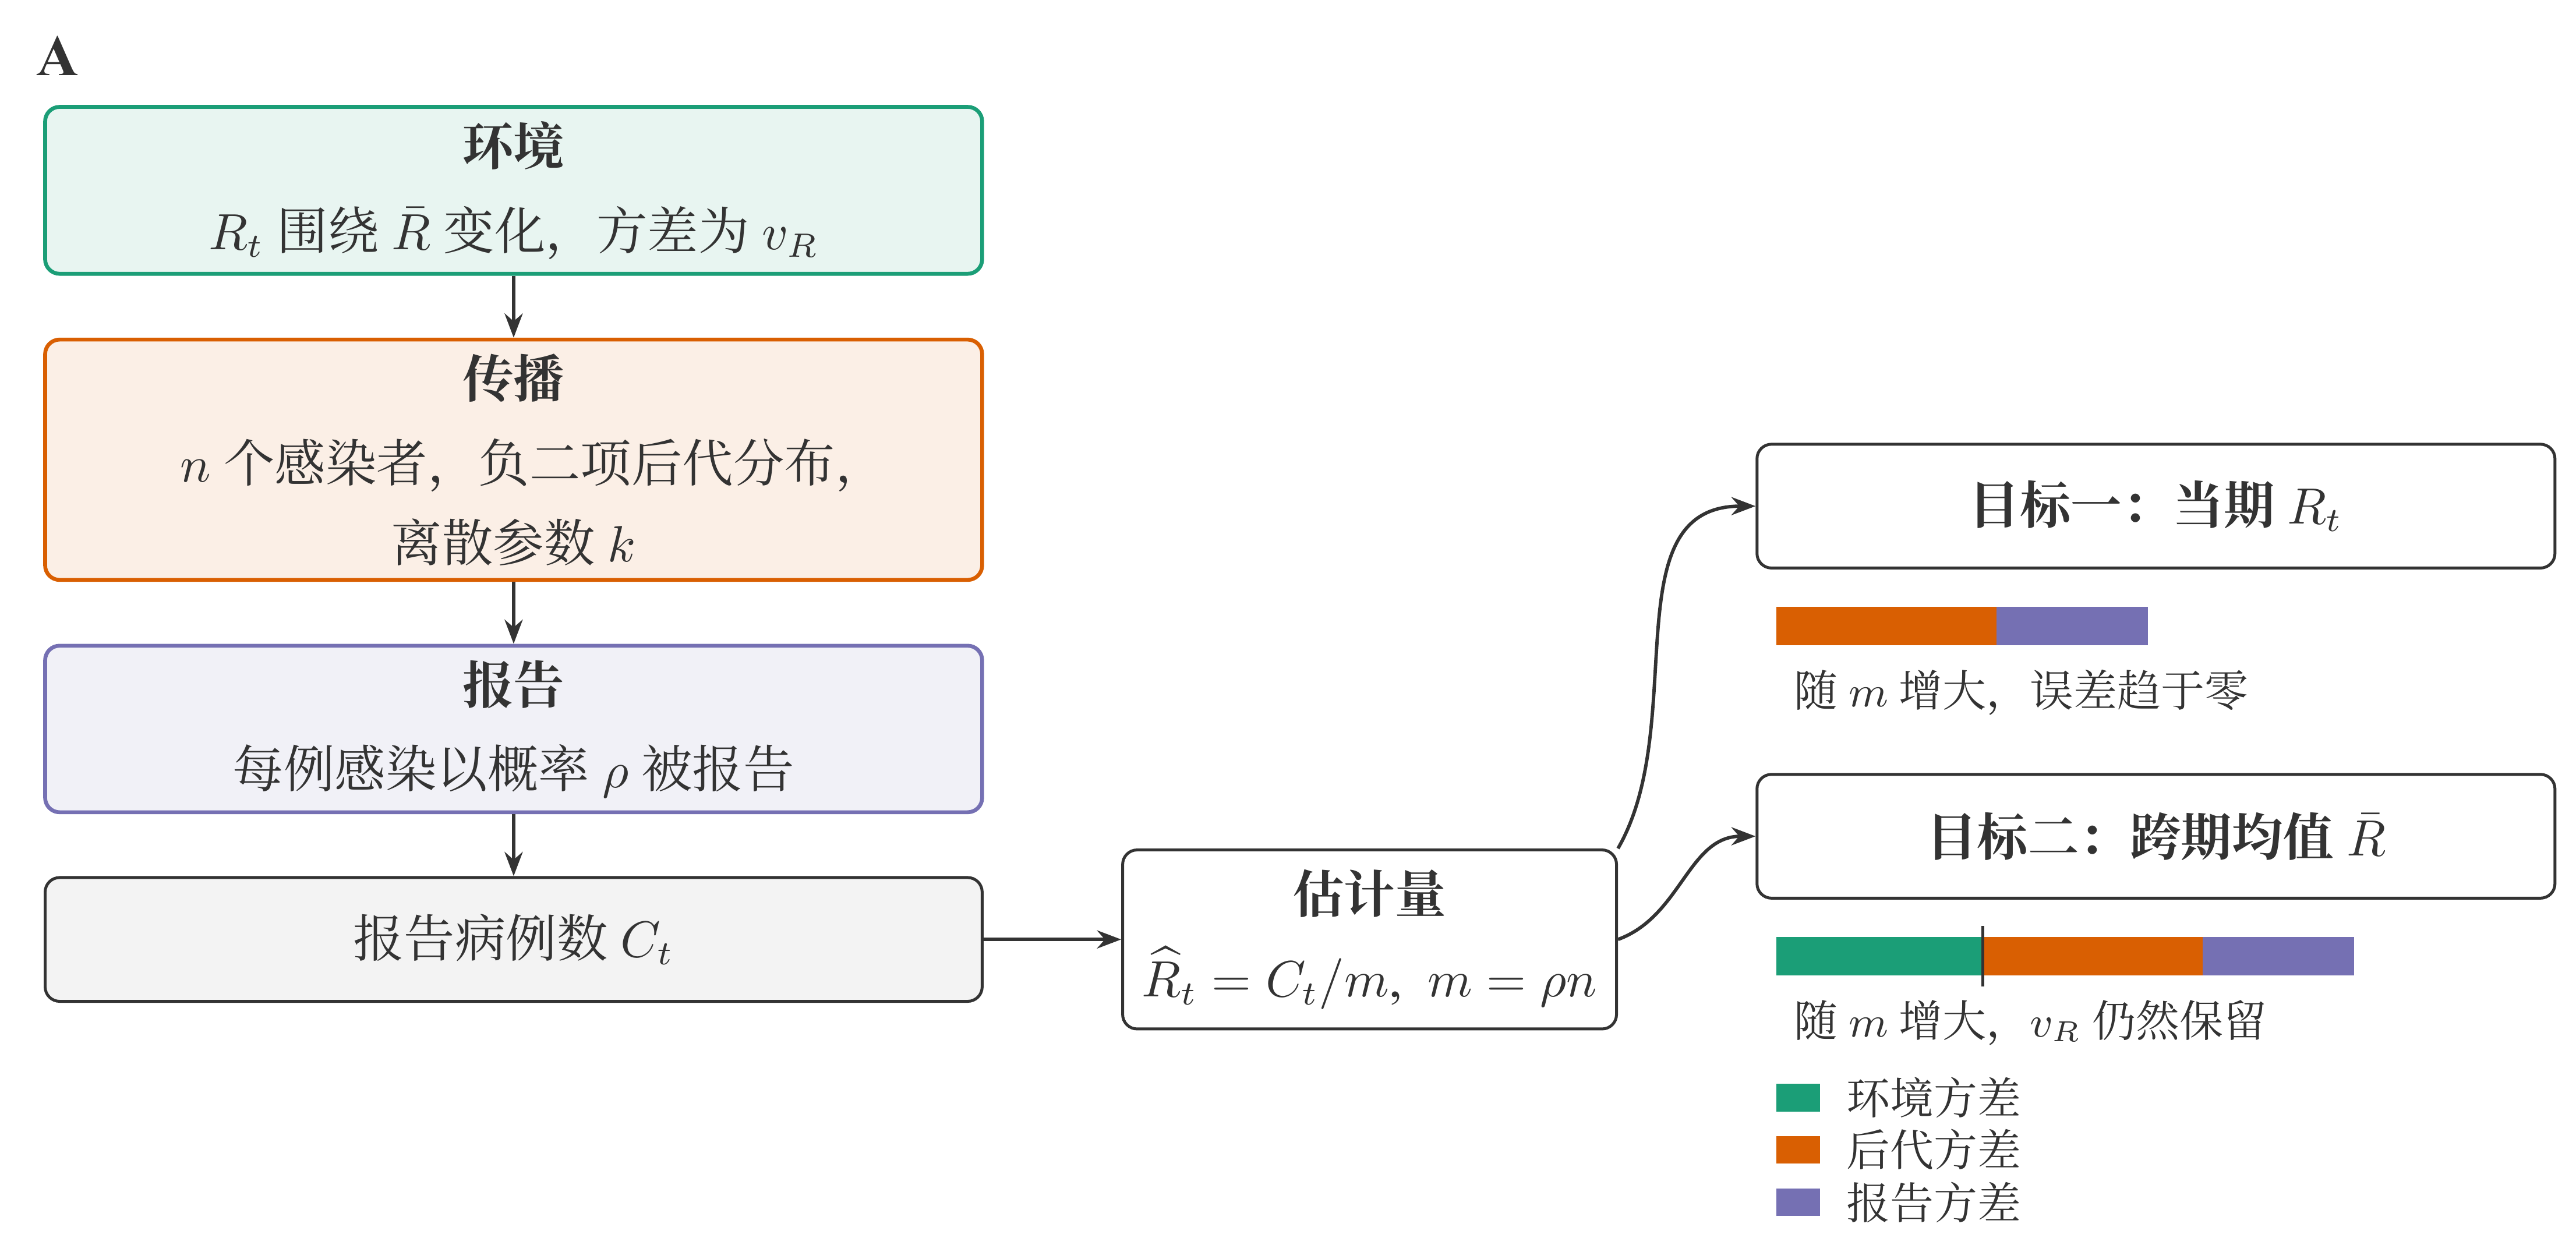
\includegraphics[width=0.86\linewidth]{figures/fig_01_schematic.png}\\[2pt]
  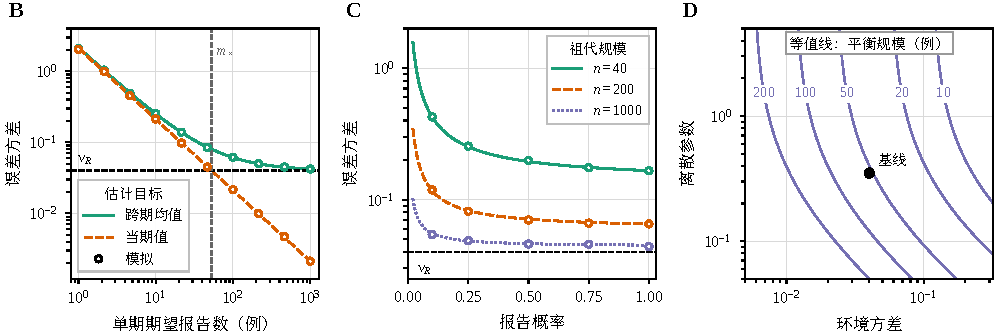
\includegraphics[width=\linewidth]{figures/fig_01_theory.pdf}
  \caption{环境变异、后代变异与报告变异对再生数尺度化估计量误差的贡献。（A）以报告病例数除以期望病例量的估计量及其两个估计目标（当期值与跨期均值）的示意图，颜色区分环境、后代与报告三类误差来源。（B）跨期均值与当期值的误差方差随单期期望报告病例数的变化；曲线为闭式解，圆点为蒙特卡罗估计及其 95\% 区间，虚线标出环境方差 $v_R$ 与平衡规模。（C）三种固定原发病例数下误差方差随报告概率的变化；完全报告时的取值为残余后代项。（D）平衡规模在环境方差与后代离散参数平面上的等值线，图中标出基线参数组合。}
  \label{fig:theory}
\end{figure}

在基线参数下（$\Rbar=1.15$，$v_R=0.04$，$k=0.35$，$\rho=0.25$；见材料与方法），抽样系数 $A=2.1232$，平衡规模为每期 $\mx=53.1$ 例报告病例（图~\ref{fig:theory}B）。当期值的误差方差在整个范围内与 $1/m$ 成比例下降，跨期均值的误差方差则逐渐趋于 $v_R$ 并保持平稳。病例量加倍时，跨期均值的误差方差在 $m=10$ 处下降 42.1\%，在 $m=\mx$ 处下降 25.0\%，在 $m=200$ 处下降 10.5\%。每个点基于 20000 次重复的蒙特卡罗估计与式~(\ref{eq:var-average}) 的偏差至多为 4.0\%。

在覆盖规模固定时提高报告概率，误差方差仍降不到 $v_R$（图~\ref{fig:theory}C）。完全报告时，原发病例数为 40、200 和 1000 的残余方差分别为 0.166、0.0652 和 0.0450，对照值为 $v_R=0.04$。在基线附近，覆盖规模按某一比例增加时误差方差的降幅，是报告概率按相同比例增加时降幅的 1.85 倍。环境方差较小且后代分布高度过离散时，平衡规模最大（图~\ref{fig:theory}D）。

\begin{figure}[t]
  \centering
  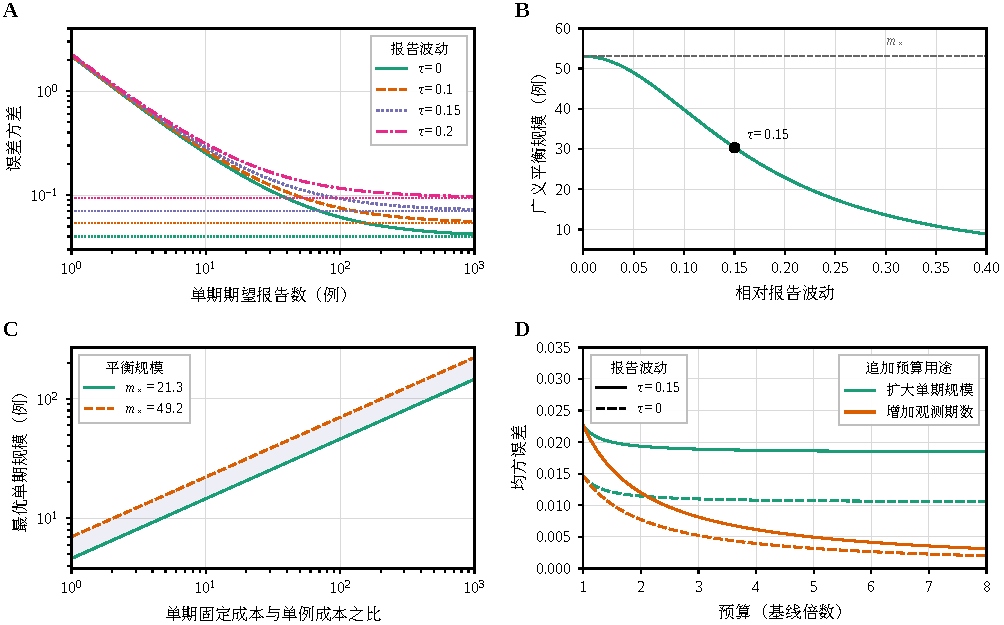
\includegraphics[width=0.92\linewidth]{figures/fig_02_heterogeneity_budget.pdf}
  \caption{报告异质性与固定监测预算的分配。（A）四种相对报告波动水平下误差方差随单期期望报告病例数的变化；点线为病例量增大时相应的极限值，由环境方差与报告方差之和决定。（B）广义平衡规模随相对报告波动的变化；虚线为无报告波动时的平衡规模，圆点为面板（D）所用的波动水平。（C）取平衡规模情景范围的两端时，单期最优报告病例数随价格比 $c_0/c_1$ 的变化；阴影带覆盖两端之间的范围。（D）环境变异与报告变异均存在自相关时，平均再生数估计量的均方误差随总预算的变化，追加预算分别用于增加单期病例数或增加时期数；实线为基线报告，虚线为标准化报告。}
  \label{fig:budget}
\end{figure}

相对报告波动 $\tau=0.15$ 使极限方差增加 $v_H=0.0307$，并使平衡规模由 53.1 例降至 30.4 例（图~\ref{fig:budget}A、B）。按流感住院设定的情景参数，潜伏平衡规模为每代 21.3--49.2 例（见材料与方法）；第~\ref{sec:res-empirical}~节给出由数据推得的潜伏值。在此范围内，式~(\ref{eq:optimal-m}) 给出的最优病例量 $m^*$ 在 $c_0/c_1=10$ 时为每期 14.6--22.2 例，在 $c_0/c_1=100$ 时为每期 46.2--70.1 例（图~\ref{fig:budget}C）。在一个假设示例中，设共有十期、每期 50 例，环境与报告均存在自相关（$\phi=\psi=0.5$），且 $\tau=0.15$，此时跨期均值的均方误差为 $22.57\times10^{-3}$，其中环境部分为 $10.40\times10^{-3}$，报告部分为 $7.88\times10^{-3}$，抽样部分为 $4.29\times10^{-3}$\,（表~\ref{tab:s7}）。病例量增至十倍时，均方误差降至 $18.71\times10^{-3}$；报告标准化使其降至 $14.65\times10^{-3}$，时期数增至四倍则使其降至 $6.17\times10^{-3}$。预算为基线的两倍时，将增量用于病例所得均方误差为 $19.35\times10^{-3}$，用于时期所得均方误差为 $11.98\times10^{-3}$\,（图~\ref{fig:budget}D）。

\subsection{表观周统计量的模拟校准}
\label{sec:res-sim}

\begin{figure}[t]
  \centering
  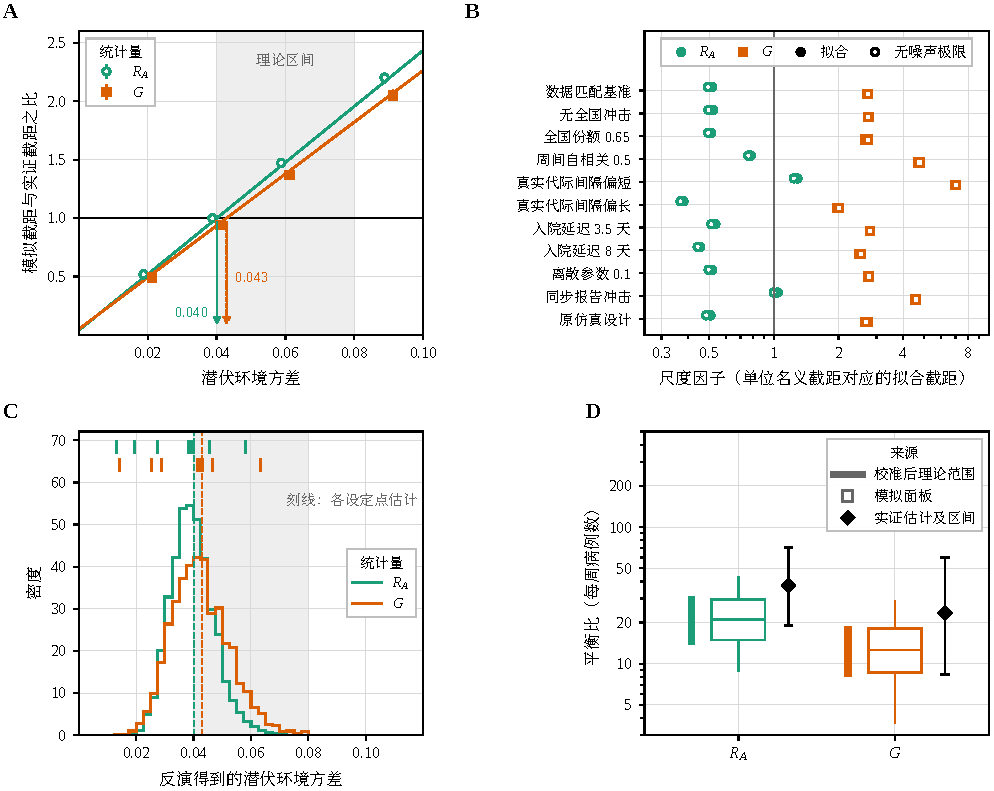
\includegraphics[width=\linewidth]{figures/fig_03_sim_inversion.pdf}
  \caption{由表观统计量反演潜在传播动态的模拟框架。（A）校准线。每个格点含 200 个模拟面板，复现观测到的流行季、窗口长度、各州规模、全国周冲击与入院延迟。拟合截距以实证截距为单位表示，虚线垂线标出各校准线与数据的交点，即隐含的潜伏环境方差 $v_R$。（B）各模拟设定下联系拟合截距与 $v_R/\Rbar^2$ 的尺度因子 $\kappa$；实心标记为拟合值，空心标记为无噪声极限。（C）数据匹配设定下隐含 $v_R$ 的分布，不确定性合并了数据的双向自助法变异与校准的蒙特卡罗误差；顶部刻线为其他设定下的点估计。（D）单个模拟面板的 $b/a$ 与校准后的理论范围，并与实证估计及其 95\% 区间比较。灰色带标出 $v_R=0.04$--0.08。}
  \label{fig:inversion}
\end{figure}

实证统计量属于表观量。加权增长比 $G$ 把多于一代的增长累积到一周之内，更新型比值 $R_A$ 则借助假定的代际间隔把周增长映射回代际尺度（第~\ref{sec:meth-stats}~节）。因此，两者的截距须先经过校准，才能与 $v_R$ 比较。我们在一套复现观测面板的模拟中建立这一校准（第~\ref{sec:meth-inversion}~节）。模拟保留四个流行季、规则窗口长度与各州初始住院量，加入承担 45\% $v_R$ 的全国周冲击以及由感染到入院的延迟，并在四个 $v_R$ 取值上各模拟 200 个面板。两种统计量的平均拟合截距均随 $v_R$ 线性上升（图~\ref{fig:inversion}A），各格点均值偏离拟合直线均不超过 0.60 个蒙特卡罗标准误。

以 $v_R/\Rbar^2$ 的倍数表示，$R_A$ 的拟合截距对应尺度因子 $\kappa=0.516$，$G$ 为 2.729，与无噪声极限 0.493 和 2.745 接近（图~\ref{fig:inversion}B）。采用 500 个独立州、每州 6 个观测周的简化设计时，无噪声极限为 0.485 和 2.698，与第一套模拟 17 个情景的中位数 0.484 和 2.68 一致。数据匹配面板同样复现了数据的相依结构：同一日历周内周损失的组内相关系数，模拟中 $R_A$ 为 0.258、$G$ 为 0.310，数据中为 0.253 和 0.310；模拟 $R_A$ 截距中的全国周份额为 0.43，观测值为 0.41。逐项改变单一设定时，$R_A$ 的 $\kappa$ 对真实代际间隔最敏感。统计量仍按 3.6 天计算时，真实均值为 2.2 天对应 $\kappa=1.287$，为 4.3 天对应 0.380。敏感程度其次的是周间传播自相关（$\phi=0.5$ 时为 0.780）和作用于报告计数的同步冲击（1.041）；全国冲击份额、入院延迟与后代离散度对它影响很小（0.454--0.535；表~\ref{tab:s8}）。

\subsection{实证截距与隐含的环境方差}
\label{sec:res-empirical}

\begin{figure}[t]
  \centering
  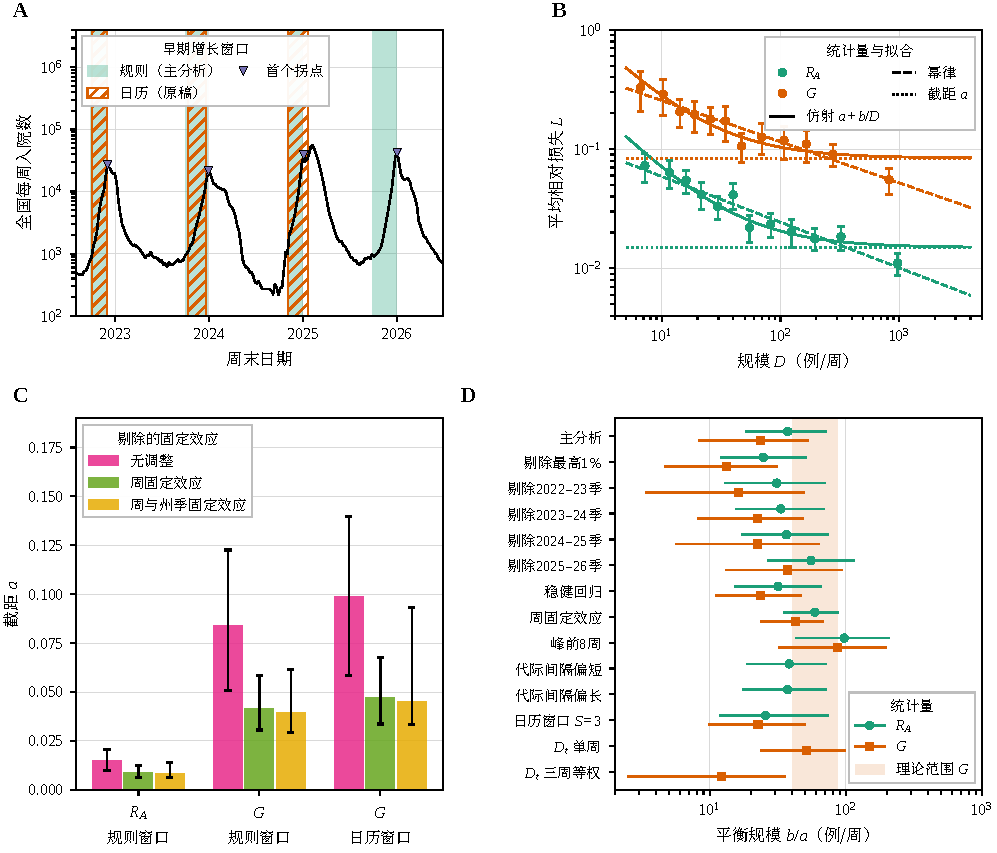
\includegraphics[width=0.86\linewidth]{figures/fig_04_empirical_loss.pdf}
  \caption{流感住院数据中两种表观周统计量的相对损失。（A）对数尺度下的全国每周住院人数；阴影为主分析采用的规则早期增长窗口，斜线为先前分析采用的日历窗口，三角形标出各流行季的首个全国拐点。（B）更新型比值与加权增长比按报告规模分箱的平均相对损失，图中绘出拟合的仿射曲线、用于比较的无截距幂律曲线以及拟合截距；分箱误差线未考虑聚类。（C）未调整、剔除全国周效应后以及进一步剔除州季效应后的截距，误差线为双向自助法区间。（D）各敏感性方案下的斜率与截距之比；阴影带为施加分母校正后增长比的未校准理论范围，校准后的范围见图~\ref{fig:inversion}D。}
  \label{fig:floor}
\end{figure}

在四个流行季按规则界定的早期增长窗口中，42 个日历周内的 1748 个州周观测给出更新型比值的截距 $a=0.0150$（95\% CI：0.0100, 0.0208）、斜率 $b=0.560$（95\% CI：0.367, 0.769）以及 $b/a=37.4$（95\% CI：19.1, 71.0；图~\ref{fig:floor}B，表~\ref{tab:s1}）。同一窗口中，加权增长比由 1756 个州周给出 $a=0.0840$（95\% CI：0.0498, 0.1248）和 $b/a=23.5$（95\% CI：8.4, 59.7）。多出的 8 个州周报告规模 $D_t$ 不低于 5，但当周住院数少于 5；$R_A$ 以单周计数为规模，因而要求当周至少 5 例。在先前分析的三个日历窗口中，增长比给出 $a=0.0991$（95\% CI：0.0569, 0.1382）和 $b/a=22.6$（95\% CI：9.0, 52.2）。两种规则窗口设定下，全部自助法重复样本的截距均为正；日历窗口下这一比例为 99.95\%。$a$ 的自助法标准差是仅对州重抽样所得标准差的 1.95--4.68 倍。

$b/a$ 在不同设定间的变化幅度，对 $R_A$ 为 3.9 倍，从剔除影响最大的 1\% 损失后的 24.7 到流行高峰周的 97.1；对 $G$ 为 7.1 倍，从分母等权时的 12.2 到流行高峰周的 86.8（图~\ref{fig:floor}D）。代际间隔变体使 $R_A$ 的 $b/a$ 变化不足 3\%。在观测到的规模范围内，无截距幂律对分箱损失的拟合与仿射形式大致相当（自助法检验 $p$ 值：$R_A$ 为 0.114，$G$ 为 0.438 和 0.418；表~\ref{tab:s2}）。本文保留仿射形式，因为其参数与命题~\ref{prop:average} 一一对应，并直接进入校准。

把各实证截距代入相应校准线，得到 $R_A$ 的隐含潜伏方差 $v_R^{\mathrm{impl}}=0.040$（95\% CI：0.026, 0.056），$G$ 为 0.043（95\% CI：0.025, 0.064）（图~\ref{fig:inversion}A、C）。区间宽度几乎全部来自实证截距的自助法变异：仅计校准误差时，$R_A$ 的区间为 0.0397--0.0406。两种统计量的尺度因子相差 5.3 倍；隐含方差之差为 $-0.003$（95\% CI：$-0.012$, 0.005），比值为 0.93（95\% CI：0.78, 1.18）。该比值的 90\% 区间为 0.81--1.13，落在 0.80--1.25 之内，因此在 5\% 水平的双单侧检验下，两个估计在 20\% 的界内等效。两个点估计都位于情景计算所用 0.04--0.08 区间的下缘，区间均向下延伸到该范围之外。在潜伏尺度上，按模拟器取值（$\Rbar=1.18$，$\rho=\rho_h=0.01$，$k=0.35$）由命题~\ref{prop:average} 得到 $R_A$ 的平衡规模为每代 30.3 例住院（95\% CI：21.7, 46.3），按每周 1.94 代折合约每周 59 例。表观值 37.4 定义在 $R_A$ 的尺度上，并不直接估计这一潜伏量。

在十种设定下，$v_R^{\mathrm{impl}}$ 介于 0.013 与 0.063 之间（图~\ref{fig:inversion}C；表~\ref{tab:s8}）。真实代际间隔的影响最大：比统计量假定的 3.6 天短时得到 0.013 和 0.014，长时得到 0.058 和 0.063。两者之差的 95\% 区间在十种设定中的九种包含零；表~\ref{tab:s8} 中的“一致”即指这种未拒绝。唯一的例外是以作用于报告计数的同步乘性冲击代替传播冲击，此时 $R_A$ 为 0.019，$G$ 为 0.029（比值 0.67；95\% CI：0.39, 0.90）。

另有三项分析检验反演的假设（表~\ref{tab:s10}）。州--季节块内相对偏差的滞后一阶自相关，$R_A$ 为 $-0.095$（95\% CI：$-0.168$, $-0.019$），$G$ 为 0.123（95\% CI：0.039, 0.201）。即使周冲击相互独立，两种统计量也会因其构造而带有自相关；独立冲击下模拟面板的均值为 $-0.074$ 和 0.114，数据分别位于第 31 和第 62 百分位。一阶系数为 0.25 时，数据位于第 3 和第 10 百分位；为 0.5 时低于全部模拟面板。季节性流感在家庭中的序列间隔估计为 3.6 天（95\% CI：2.9, 4.3）\citep{cowling2009estimation}。真实代际间隔均值为 2.9 天时，隐含方差对 $R_A$ 为 0.026（95\% CI：0.017, 0.036），对 $G$ 为 0.027（95\% CI：0.016, 0.040）；为 4.3 天时为 0.058 和 0.063。数据的自相关在 2.9 天的模拟面板中位于第 2.5 和第 9 百分位，在 4.3 天时位于第 80 和第 92 百分位，因此并不支持较短的间隔。不过，较短的间隔能复现实证 $b/a$：在最接近其隐含方差的模拟取值 $v_R=0.02$ 处，数据位于模拟 $b/a$ 分布的第 52.5 和第 58 百分位。周住院数过度离散、方差均值比为 1.5 或 2.0 时，隐含方差保持在 0.039--0.045，而 $v_R=0.04$ 处模拟的 $b/a$ 对 $R_A$ 由 28.0 升至 68.0 和 81.0，对 $G$ 由 16.2 升至 40.2 和 48.4。这些设定下两种统计量的滞后一阶自相关都低于数据，因此数据更支持小于方差均值比 1.5 的过度离散。

在各统计量自身的尺度上，取 $v_R\in\{0.04,0.08\}$、$k\in\{0.2,0.5\}$ 与入院概率 $\rho_h\in\{0.0056,0.021\}$ 的八种组合，校准后的理论 $b/a$ 对 $R_A$ 为 13.9--31.1，对 $G$ 为 8.0--18.8（图~\ref{fig:inversion}D）。实证点估计 37.4 和 23.5 位于这两个范围之上，其 95\% 区间与之重叠。单个模拟面板的比值离散较大，95\% 落在 $R_A$ 的 8.8--42.7 和 $G$ 的 3.6--28.6 之间；实证值分别位于这两个分布的第 93 和第 91 百分位。

\subsection{监测不确定性的多尺度分解}
\label{sec:res-multiscale}

截距包含同一日历周内各州共有的分量和各州特有的分量（图~\ref{fig:floor}C；表~\ref{tab:s2}）。剔除全国周效应后，规则窗口中 $R_A$ 的 $a$ 下降 41\%（95\% CI：12, 59），$G$ 下降 51\%（95\% CI：21, 67），日历窗口中 $G$ 下降 52\%。再剔除州季效应，截距变化很小。两项调整后 $R_A$ 的截距为 0.0083（95\% CI：0.0064, 0.0141），且在所有设定中州季分量的区间均包含零。同一日历周内损失的组内相关系数，$R_A$ 为 0.253，$G$ 为 0.310。自助法呈现同样的结构。仅对周重抽样时，$\hat{a}$ 的标准差 $R_A$ 为 0.0021，$G$ 为 0.0158，分别是仅对州重抽样的 1.46 和 1.87 倍；双向重抽样则为 0.0028 和 0.0193。

全国周分量在同一周内进入每个州的损失。某州住院数增加只能缩小该州的计数项，对多州取平均只能缩小州特有项，两者都消除不了共有分量，只有增加观测周数才能把它平均掉。随机抽取 $J$ 个州合并平均周偏差时，$R_A$ 的方差在 $J=5$、10 和 51 时分别降至单州的 0.39、0.31 和 0.25，$G$ 降至 0.43、0.36 和 0.31（图~\ref{fig:design}C）。这些值逐渐逼近全国周分量，后者对 $R_A$ 为单州方差的 0.23，对 $G$ 为 0.29；$R_A$ 在 $J=33$、$G$ 在 $J=25$ 时与之相差不到 10\%，与式~(\ref{eq:pooling}) 对部分同步变异的预测一致。

\subsection{强制报告与自愿报告制度}
\label{sec:res-reporting}

\begin{figure}[t]
  \centering
  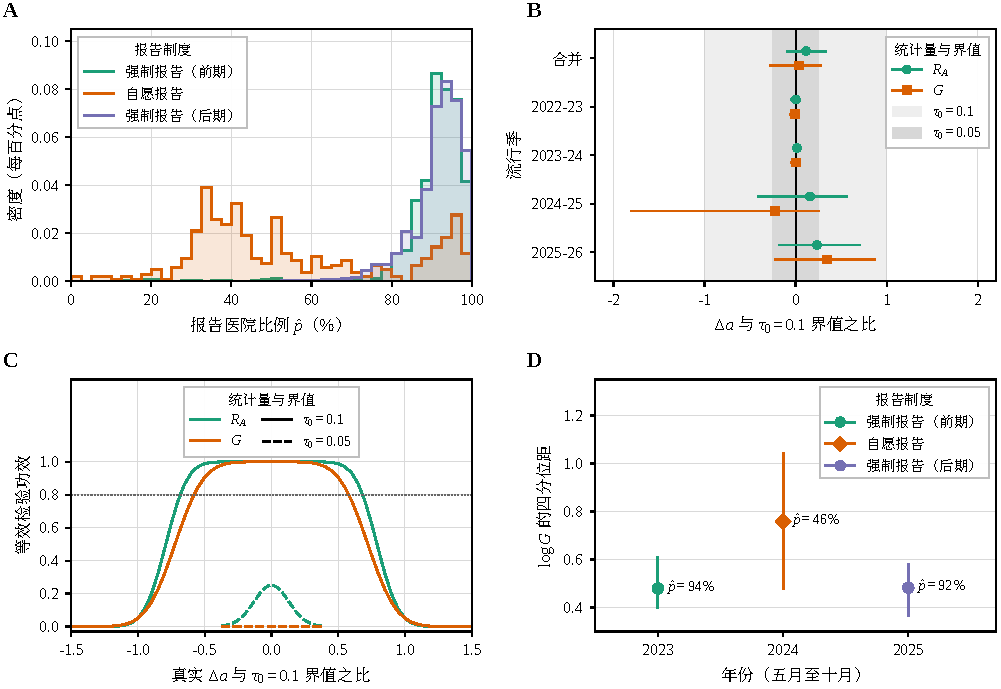
\includegraphics[width=0.86\linewidth]{figures/fig_05_reporting.pdf}
  \caption{报告完整度与经验截距。（A）三种报告制度下报告流感住院人数的医院占比分布。（B）统计量按报告覆盖率调整后截距的变化，分别给出合并估计与逐季估计及其 90\% 配对自助法区间；各统计量均以自身的等效界为单位表示，阴影带为两个报告波动阈值所对应的等效界。（C）两种统计量在两种等效界下双单侧等效检验的功效随真实变化量的变化，图中给出常规功效参照线。（D）三个日历年五月至十月增长比对数的四分位距；自愿报告的年份突出显示，标注为报告完整度中位数。}
  \label{fig:reporting}
\end{figure}

在报告规模不低于 5 的州周中，报告医院占比的中位数在第一个强制报告期为 92.3\%，在自愿报告期为 45.7\%，恢复强制报告后为 92.9\%（图~\ref{fig:reporting}A）。规则窗口内的中位数为 93.7\%，79.8\% 的州周至少有 90\% 的医院报告。在这些窗口中，按报告占比调整统计量后，$R_A$ 的截距变化 $\Delta a=0.29\times10^{-3}$\,（90\% CI：$-0.22\times10^{-3}$, $0.85\times10^{-3}$），$G$ 的截距变化 $0.37\times10^{-3}$\,（90\% CI：$-2.83\times10^{-3}$, $2.81\times10^{-3}$）（图~\ref{fig:reporting}B；表~\ref{tab:s3}）。以相对报告波动 $\tau_0=0.10$ 设定等效界，两项变化均与零等效。按式~(\ref{eq:tost})，等效界取决于各统计量的样本均值，折合为 $R_A$ 截距的 17\%（95\% CI：12, 25）和 $G$ 截距的 12\%（95\% CI：8, 20）。实测变化占 $R_A$ 截距的 2.0\%（95\% CI：$-2.4$, 6.1；单侧 95\% 上界 5.3\%），占 $G$ 截距的 0.4\%（95\% CI：$-4.4$, 4.0；上界 3.5\%）；逐季检验中，$R_A$ 的四个流行季全部等效，$G$ 有三个等效。取 $\tau_0=0.05$ 时，等效界约为截距的 4\% 和 3\%，两项变化均未达到等效，真实变化为零时检验功效对 $R_A$ 为 0.25，对 $G$ 为 0（图~\ref{fig:reporting}C）。

报告完整度明显偏低的对照只有自愿报告期这一个。五月至十月期间，$\log G$ 的四分位距在自愿报告的 2024 年为 0.759，2023 年为 0.479，2025 年为 0.483（图~\ref{fig:reporting}D；表~\ref{tab:s4}）。2024 年与 2023 年之比为 1.58（95\% CI：0.95, 2.23），与 2025 年之比为 1.57（95\% CI：0.95, 2.39），作为安慰剂的 2025 年与 2023 年之比为 1.01（95\% CI：0.72, 1.25）。这三年同期的报告规模中位数相近（15.6、16.6 和 16.2 例），按报告规模匹配州周后，两个比值为 1.68 和 1.58。按日历月匹配时，比值中位数为 1.33，十二组月份--年份比较中有九组大于 1。COVID-19 住院数据中，2024 年相对 2023 年和 2025 年的比值为 1.62 和 1.18；RSV 住院数据中，相对 2025 年的比值为 1.36。在有实验室数据的 44 个州中，实验室 $R_A$ 与住院 $R_A$ 的相关系数 $r=0.31$，实验室部分占住院截距的 0.230（95\% CI：0.043, 0.418）。

\subsection{收益递减与监测设计}
\label{sec:res-design}

\begin{figure}[t]
  \centering
  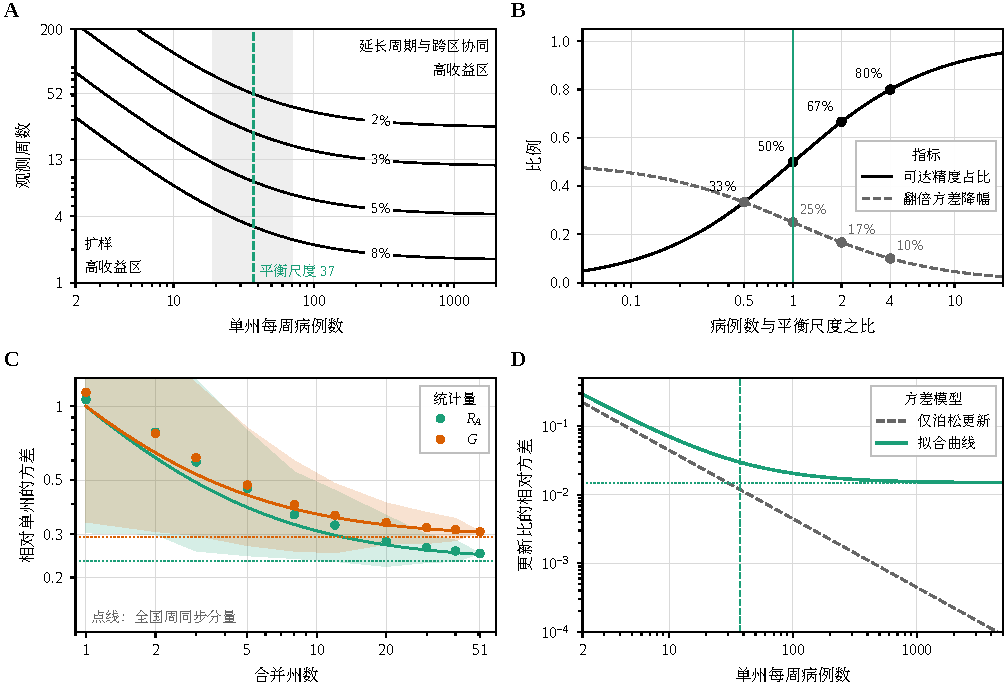
\includegraphics[width=\linewidth]{figures/fig_06_design_nomogram.pdf}
  \caption{监测设计列线图。（A）单州平均更新型比值 $R_A$ 的相对标准误达到 2\%--8\% 所需的观测周数随每周住院数 $m$ 的变化，按统计量自身尺度计算且不计州内自相关；虚线为平衡规模 $\mx=b/a$，灰带为其 95\% 区间。虚线左侧，增加病例带来大部分收益；右侧等值线趋平，增加观测周数或区域带来大部分收益。（B）可达精度占比 $m/(m+\mx)$ 以及 $m$ 加倍一次带来的方差降幅。（C）对 $J$ 个州合并后平均周偏差的方差，以单州为 1，分别给出 $R_A$ 与增长比 $G$；圆点与阴影带来自随机抽取的州子集，点线为全国周分量。（D）$R_A$ 的相对方差：仅含泊松更新方差的模型与拟合的 $a+b/m$ 比较。}
  \label{fig:design}
\end{figure}

在 $V(m)=a+b/m$ 下，病例量不受限时可达精度中能够实现的份额为 $m/(m+\mx)$，$m$ 加倍一次使方差降低 $\mx/[2(m+\mx)]$（命题~\ref{prop:average}）。$m$ 为 $\mx$ 的 0.5、1、2 和 4 倍时，这一份额依次为 33\%、50\%、67\% 和 80\%，由这些位置再加倍一次，方差依次下降 33\%、25\%、17\% 和 10\%；要实现可达精度的 90\%，需要 $m=9\mx$（图~\ref{fig:design}B）。以 $R_A$ 的实证 $\mx=37.4$ 和 $G$ 的 23.5 计，规则窗口中分别有 55\% 和 65\% 的州周位于平衡规模之上。对单个州而言，使平均 $R_A$ 达到给定相对标准误所需的观测周数在住院数低于 $\mx$ 时随住院数增加而迅速减少，高于约 $4\mx$ 后几乎不再变化（图~\ref{fig:design}A）。取实证平衡规模与成本比 $c_0/c_1=10$，最优病例量 $R_A$ 为 $m^*=19.4$（95\% CI：13.8, 26.6），$G$ 为 15.3；$c_0/c_1=100$ 时为 61.2 和 48.4。

拟合方差与泊松更新模型不同。后者估计误差方差为 $\Rbar/m$，不含随 $m$ 增大而保留的项（图~\ref{fig:design}D）。在 $R_A$ 的表观尺度上，拟合斜率是泊松值 0.446 的 1.25 倍，拟合方差在 $m=22$ 时为泊松方差的两倍，在 $m=261$ 时为十倍；在命题~\ref{prop:average} 的潜伏尺度上取 $v_R=0.040$，相应位置为 $m=28$ 和 $m=262$。

流行季数量限制了对季间变异的任何估计（图~\ref{fig:seasons}）。$R_A$ 的分季截距依次为 0.0137、0.0062、0.0127 和 0.0225，随机效应均值为 0.0125（95\% CI：0.0022, 0.0227），$I^2=0.47$（表~\ref{tab:s5}）。$G$ 的随机效应均值在规则窗口中为 0.0619（95\% CI：0.0066, 0.1171），在日历窗口中为 0.0735（95\% CI：$-0.0558$, 0.2028）。季间方差的任何无偏估计，其相对标准误在三个流行季时至少为 1.00，四个流行季时至少为 0.82（推论~\ref{cor:season}）。对于流感、COVID-19 和呼吸道合胞病毒（RSV），替代分母权重下的截距比均呈现 $q_1<1<q_2$，例如流感在日历窗口中 $q_1=0.688$，$q_2=1.539$（表~\ref{tab:s6}）。在只有报告噪声与流行增长、没有环境变异时，日历窗口中 $q_1$ 的范围为 0.63--0.89，$q_2$ 为 1.13--1.58，因此这一排序无法区分机制。40 项单侧检验中，校正前有 21 项显著，经 Benjamini--Hochberg 校正后有 18 项显著，经 Holm 校正后有 10 项显著，全部来自流感，其中没有一项是针对偏离零假设范围的检验。
